\section{System Design and Implementation}
\phantomsection
\subsection{Requirements}
        \subsubsection{Functional requirements}
            The software should run on NAO. NAO should be able to sort a set of objects. That means NAO should be able to move. This also means that NAO should be able to ``see''. The last thing is that he should also be able to ``think'' in order to sort which object goes where. Now these very brief requirements would be expanded until the clear goals are defined. 
            Requirements:
            \begin{enumerate}[topsep=2pt, partopsep=0pt,itemsep=0pt,parsep=1pt]
                \item Move:
                    \begin{enumerate}[topsep=1pt, partopsep=0pt,itemsep=0pt,parsep=1pt]
                        \item walk;
                        \item stand up -- robot might start his activity sitting, so it is needed to stand him up;
                        \item sit down -- it is safe to leave the robot in the end in sitting state;
                        \item turn with the whole body to a relative degree;
                        \item take a custom position to grasp an object;
                        \item return to a standard position after grasping;
                        \item close hand -- grasp something;
                        \item open hand -- release something;
                        \item rise hand -- give the object to someone;
                        \item lower hand;
                        \item turn head to a relative direction -- look towards something.
                    \end{enumerate}
                \item See:
                    \begin{enumerate}[topsep=1pt, partopsep=0pt,itemsep=0pt,parsep=1pt]
                        \item take an image with the camera;
                    \end{enumerate}
                \item Think:
                    \begin{enumerate}[topsep=1pt, partopsep=0pt,itemsep=0pt,parsep=1pt]
                        \item compute distance -- ``feel'' how far is an object from the image;
                        \item detect objects:
                            \begin{itemize}[topsep=1pt, partopsep=0pt,itemsep=0pt,parsep=1pt]
                                \item[--] subtract background;
                                \item[--] eliminate shadow.
                            \end{itemize}
                        \item sort objects:
                            \begin{itemize}[topsep=1pt, partopsep=0pt,itemsep=0pt,parsep=1pt]
                                \item[--] extract features -- prepare for clustering;
                                \item[--] cluster objects -- group them.
                            \end{itemize}
                    \end{enumerate}
                \item Interact:
                    \begin{enumerate}[topsep=1pt, partopsep=0pt,itemsep=0pt,parsep=1pt]
                        \item receive commands -- speech commands;
                        \item execute commands -- react to them;
                        \item speak;
                        \item recognize speech;
                        \item detect audio source -- detect where is the speaker.
                    \end{enumerate}
            \end{enumerate}
        \subsubsection{Non-functional requirements}
            \noindent These requirements are dictated by circumstances or are implied by functional requirements. 
            \begin{enumerate}[topsep=2pt, partopsep=0pt,itemsep=0pt,parsep=1pt]
                \item The programming language required is C++ because this is the only one which can be executed locally on NAO;
                \item Project should be cross-platform: run both on Linux and Mac OS X;
                \item For better object detection take two pictures: one of plain background and the second one already with objects;
                \item Use the available libraries and SDK-s and their functionality;
                \item Use Qt Creator as IDE because this one is recommended and \verb|qibuild| can create projects for it;
                \item Build on Linux because cross-compilation feature is available only in Linux version of NAO SDK. So to build a project which would run on robot Linux is required;
                \item Store all images in OpenCV internal format, since this is the format received from the camera and good for all image processing algorithms.
            \end{enumerate}\itemsep0pt

\addtocontents{toc}{\protect\newpage}

    \subsection{Compilation process}
            NAO robot runs a Linux-like operating system. There are two ways to execute a program on NAO: \textbf{local execution and remote execution}. In the first case, all the code runs on NAO and this is the fastest possibility to retrieve data from \verb|ALMemory| module where all the values of sensors are stored. To deploy something on NAO, the code should be written in C++. Having your code on a PC or laptop, it is needed to build the project for a different machine -- for the robot. This action is called \textbf{cross-compilation}: compilation and creation of an executable for a platform other than the one on which compiler is running. Such a functionality is available only in the SDK for Linux operating system (though NAO SDK is available also for Mac OS X and Windows). Remote execution is running the executable on a different machine, while accessing robot functionality through network. This functionality is implemented with Proxy pattern in mind -- in code a proxy to a certain module is created, then the functionality of this module is used. This way is slower in terms of accessing NAO's modules but it has the advantages of using a more powerful processor, since the processor on robot is quite robust in terms of processing power. During this project, only remote execution was used.

            NAO SDK comes with a tool for building. It is similar to \verb|make|. It is called \verb|qibuild|. \verb|qibuild| manages dependences between projects and supports cross-compilation. Below are presented the needed commands to create and build a project. The following steps need to be performed:
            \begin{enumerate}[topsep=2pt, partopsep=0pt,itemsep=0pt,parsep=1pt]
                \item create a worktree: \verb|qibuild init|
                \item create a project: \verb|qibuild create foo|
                \item configure and make the project: \verb|qibuild configure -c mytoolchain foo|
                \item        \verb|qibuild make -c mytoolchain foo|
                \item to open a project in an IDE (for example, Qt Creator): \verb|qibuild open foo|
            \end{enumerate}


        \subsection{Object-oriented design}

        Object Oriented Programming is perhaps the most successful approach to software development. Moreover, the foundation on which this program should be build is written in OOP style as well, both NAO SDK and OpenCV. That is why such an approach would be used here. But before designing this system, there is need to explore the available SDK-s first. That way it would be clear what is already implemented and how this can be used in current project.

    \subsubsection{NAOqi API}

        NAOqi is the name of the main software that runs on the robot and controls it. The NAOqi Framework is the programming framework used to program NAO. It answers to common robotics needs including: parallelism, resources, synchronization, events. This framework allows homogeneous communication between different modules (motion, audio, video), homogeneous programming and homogeneous information sharing, \cite{naoDocumentation}. It runs on robot but also can be installed on a different machine to be run on a simulator. The NAOqi API is currently available in at least 8 languages. Apart from some minor language-specific differences, the API is mostly the same across all languages, allowing you to bring knowledge from one language to another. The C++ framework is the most complete framework. It is the only framework that lets you write real-time code, running at high speed on the robot (with loops of less that 10 ms, for instance).

    All the functionality of NAOqi is separated into modules. Each module is composed of concrete classes which implement the specific functionality. The modules are:
        \begin{enumerate}[topsep=5pt, partopsep=0pt,itemsep=3pt,parsep=1pt]
            \item Core -- NAOqi comes with a list of core modules that are always available. Every module comes with a list of default methods.
            \item Motion -- the \verb|ALMotion| module provides methods which make NAO move.
            \item Audio -- this represents the audio software components that run on robot.
            \item Vision -- for vision.
            \item Sensors -- deals with bumpers, tactile hands, tactile head and chest button. Also includes data from battery infrared sensors, sonars and laser.
            \item Trackers -- the Tracker modules allow you to make NAO track targets (a red ball or a face). The main goal of these modules is to establish a bridge between target detection and motion in order to make NAO keep in view the target in the middle of the camera.
            \item DCM -- Device Communication Manager, is a Hardware Abstraction Layer.
        \end{enumerate}
        Not all of these modules were used. Next the specific classes important for this project would be described and their functionality.
        \verb|ALError| is used to send exception. All NAOqi errors are based on exceptions. All user commands should be encapsulated in a try-catch block. Example of usage:
        \renewcommand{\thelstlisting}{\thesection.\arabic{lstlisting}}
        \lstinputlisting[language=C++, caption={Try-catch block in NAOqi}, label=list1]{../SrcCode/tryCatch.cpp}
\vspace{5mm}
        The module \verb|ALTextToSpeechProxy| is used to make NAO say something. As it can be observed, this and most of the following modules would have the postfix \verb|Proxy| which signifies the fact that this class acts like a proxy to a real speech module which runs on robot (while this module is used for remote execution). Example of usage:
        \lstinputlisting[language=C++, caption={Text-To-Speech functionality}, label=list2]{../SrcCode/tts.cpp}
\vspace{5mm}
        \verb|ALMotionProxy| is used for generic movements of any part of the robot's body, as well as for position retrieval. As a general pattern, all \verb|Proxy| classes take as an argument a \verb|std::string| which is the robot's IP, so the module could connect to the robot. Here's an example how to get the robot's position in space:
        \lstinputlisting[language=C++, caption={Getting robot's position}, label=list3]{../SrcCode/motion.cpp}
\vspace{5mm}
        \verb|ALRobotPostureProxy| is a class which implements the functionality of getting robot into one of the predefined postures. There are 8 predefined postures, like \verb|Stand| or \verb|Sit|. The method \verb|goToPosture| is the most important one, which takes care of other things as well:
        \lstinputlisting[language=C++, caption={Changing robot's posture}, label=list4]{../SrcCode/posture.cpp}
\vspace{5mm}
        \verb|ALNavigationProxy| implements safe walking. It subclasses \verb|ALMotionProxy|, using the generic movement in the back, but also checks for an obstacle thanks to the sensors. If there is an obstacle, the robot stops. 
        \lstinputlisting[language=C++, caption={Safe walking}, label=list5]{../SrcCode/walking.cpp}
\vspace{5mm}
        \verb|ALValue| is a generic wrapper of data in NAOqi. Numerous methods return the information stored in this form, or take it as a parameter.
        \verb|ALVideoDeviceProxy| is the accessor to the NAO's camera. To get an image remotely, one must first subscribe to the camera as a client, then ask for an image:
        \lstinputlisting[language=C++, caption={Getting images from camera remotely}, label=list6]{../SrcCode/getImage.cpp}
\vspace{5mm}
        \verb|ALMemoryProxy| is the class which gives the access to all the data from sensors and robot parts. The method \verb|getData| takes a string as an argument specifying which data to return. The next example shows how to retrieve data related to speech recognition of certain words:
        \lstinputlisting[language=C++, caption={Accessing NAO's memory}, label=list7]{../SrcCode/memory.cpp}
\vspace{5mm}
        But to start the speech recognition we need to first set some parameters and use the \\\verb|ALSpeechRecognitionProxy| class:
        \lstinputlisting[language=C++, caption={Speech recognition functionality}, label=list8]{../SrcCode/speech.cpp}
\vspace{5mm}
        Because NAO has 4 microphones, it can compute with some limited precision where the source of the sound is located. This functionality is built in \verb|ALAudioSourceLocalizationProxy| class.
        \lstinputlisting[language=C++, caption={Sound localization functionality}, label=list9]{../SrcCode/soundLocalization.cpp}
        \vspace{5mm}
        This is basically all the functionality of the robot which is needed for this project. Next, an analysis of OpenCV used methods and classes is presented.


    \subsubsection{OpenCV API}

        OpenCV was discussed in the previous chapter. This section briefly summarizes the used API. 
        The basic data structure used throughout the whole framework is \verb|cv::Mat|. In order to get access to it, there should be included \verb|opencv2/opencv.hpp| header file, but other OpenCV headers contain these primary definitions as well. A \verb|Mat| represents a matrix. It offers the implementation of basic matrix operations, both with other matrices and with scalar numbers as well. It is the structure used to store data of all the images. Besides \verb|Mat|, \verb|cv::Point2d| is used for representation of points and pairs of numbers. The structure \verb|cv::Rect| was used to represent a bounding rectange of a subimage and in object detection. To read an image form the file system call: 

        % the function \verb|cv::imread| is called with first parameter a string with file location and second parameter a constant indicating in which format should the file be read: 

         % The core functionality of OpenCV is given in \verb|opencv2/core/core.hpp| file.

        \verb|mat = cv::imread( BACKGROUND_IMAGE, CV_LOAD_IMAGE_COLOR );|

         \noindent While performing the object detection the following modules are used: 
        \begin{enumerate}[topsep=5pt, partopsep=0pt,itemsep=3pt,parsep=1pt]
            \item image processing module, defined in     \verb|opencv2/imgproc/imgproc.hpp|;
            \item GUI model (for windows and outputs),
            defined in \verb|opencv2/highgui/highgui.hpp|;
            \item the background segmentation algorithm,
            defined in \verb|opencv2/video/background_segm.hpp|;
        \end{enumerate}\itemsep0pt

        To show an image in a window the following functions would be used:
        \lstinputlisting[language=C++, caption={Show image functionality}, label=list10]{../SrcCode/showImage.cpp}
\vspace{5mm}
        To subtract the background, first a matrix mask is defined. It will contain the differences between background and foreground. Then an instance of \verb|BackgroundSubtractorMOG2| class is created and some parameters are adjusted: After that, the images of background and foreground are fetched to the instance and the mask is received:
        \lstinputlisting[language=C++, caption={Background subtraction}, label=list11]{../SrcCode/subtraction.cpp}
\vspace{5mm}
        The access of a pixel itself in a gray-color image is done in the following way:

        \verb|mask.at<uchar>(i,j) = 0;| 

        \noindent where \( i, j \) represent the row and column in the matrix. There is just one value -- the intensity. To access a pixel of a RGB image a similar procedure is done:

         \verb|cv::Vec3b pixel = mat.at<cv::Vec3b>(x,y);| 

         \noindent but here one pixel is a 3-dimensional vector. To convert an image from RBG to  gray scale it is possible to call:

        \verb|cvtColor( recolored_src, src_gray, CV_BGR2GRAY );|

        \noindent To blur an image simply call: 

        \verb|blur(src_gray, src_gray, cv::Size(3,3) );| 

        \noindent To detect a threshold the following code is executed:

        \verb|threshold( gray, threshold_output, i, 255, cv::THRESH_BINARY );| 

        \noindent To find contours: 
        \lstinputlisting[language=C++, caption={Finding contours}, label=list12]{../SrcCode/contours.cpp}
\vspace{5mm}
       Next the contours can be approximated to polynomials:

        \verb|approxPolyDP( cv::Mat(contours[i]), contours_poly[i], 3, true );| 
       
         \noindent and a polynomial might be bounded by a rectangle:

         \verb|boundingRect( cv::Mat(contours_poly[i]) );|

        \noindent To use the OpenCV built-in K-means clustering algorithm:
        \lstinputlisting[language=C++, caption={K-means clustering}, label=list13]{../SrcCode/clustering.cpp}

    \subsubsection{Objects and classes}

        Before starting the design of the system and defining the classes it is preferable to first look which objects there are, then group them into classes. There is a robot. So there should be a class \verb|NAO|. There are real objects, like a duck or a ball or a chess figure; so there should be a class which reassembles an object. On NAO, there is the camera, but when the project runs on Mac OS X the images are retrieved from the file system. Thus there should be a class which generalizes the functionality, let's say \verb|ImageFetcher|. The project deals with images, there is an object which can cluster, one which can move, one which can compute the distance, other which can speak and listen. All these are integrated in NAO. So we would have some kind of composition. Many of the above responsibilities can be performed by a \verb|Head|. But a class should have only one responsibility. So the head would unify all these processes. Going out from the rule of thumb that one class should have only one responsibility, the following classes were defined:

        \begin{enumerate}[topsep=3pt, partopsep=0pt,itemsep=1pt,parsep=1pt]
            \item \verb|Speech|;
            \item \verb|CustomMoves|, \verb|Locomotion|, \verb|SpaceOrientation| -- for locomotion;
            \item \verb|Image|, \verb|Object|, \verb|ObjectDetector|;
            \item \verb|AbstractImageFetcher|, \verb|Camera|, \verb|ImageFetcherOnOSX|;
            \item \verb|AbstractClusterAlgorithm|, \verb|KMeansClusterAlgorithm|;
            \item \verb|Head|, \verb|NAO|, \verb|Factory| (implements the corresponding design pattern).
        \end{enumerate}\itemsep0pt


    \subsubsection{Relationships between classes}
        The following diagrams present the structure of the system. They present the classes from which this system is composed and the relationship between them. They also show the dependencies. The use case diagrams of the system can be found in the appendix A.    
        In figure \ref{image} The \verb|Image| class is just a wrapper of OpenCV \verb|cv::Mat| class with additional helper methods. The image of objects or background is obtained from some \verb|AbstractImageFetcher| -- is it a camera, on robot or just some pictures from the filesystem on Mac OS X. All the classes which access NAO SDK modules need to know the robot's IP. This one is given as argument to the constructor, as a string (see \verb|Camera| class). To get an image from the robot using the proxy the corresponding SDK calls are performed. Because the SDK is available only on Linux, a platform check is performed: \verb|#ifdef __linux__| then the SDK is used. The center of the image is not contained in an attribute, but is computed every time its getter is called from \verb|boundingRect|. Each class has also the copy constructor implemented and assignment operator overloaded. Besides that, the stream operator is overloaded as well. The stream operator ``streams'' all the members of the corresponding class. From the diagram we can see that the class \verb|Image| has private attributes \verb|matrix| and \verb|boundingRect| and it also knows about \verb|cv::Point2d|.
         

        \begin{figure}[h!]
            \centering
            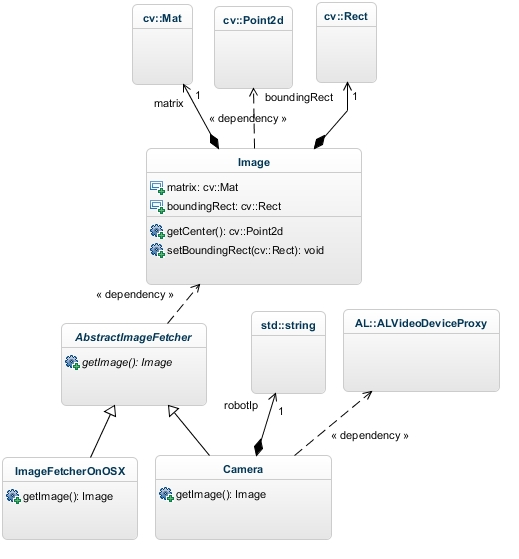
\includegraphics[scale=0.9]{21.eps} 
            \caption{Image Fetcher classes}
            \label{image}
        \end{figure}
% \newpage
        In figure \ref{detector} the \verb|Object| class is represented by an image. It has a position in space and in the scope of this project it has a property called \verb|group|, which is the label received after clustering. The class \verb|ObjectDetector| has just one public method: \verb|detectObjectsFromImage()|. All the intermediary steps of detection should be implemented in private methods. The detection algorithm implemented in \verb|ObjectDetector| class is presented in figure \ref{activity1}. This algorithm is simple and it contains a uniform flow of steps. Behind the private methods shown in the detector, there are operations like checking if a rectangle is inside another rectangle or recoloring a set of pixels to the color of background. Some constants of minimal and maximal area of acceptable objects are also defined in the header file. The class \verb|BoundingRect| has properties like top left corner and bottom right one, rectangle width and height. In the start, the detection was implemented in such a way that the objects would be extracted from just one image. It took into account notable differences between the colors on neighbor pixels, but such an implementation would never work on a background like chess board. It proved to be erroneous, because it is difficult to make sense what is the background just from one image. The class \verb|ObjectDetector| ``knows'' how to detect objects of class \verb|Object|. It also uses internally \verb|BackgroundSubtractorMOG2| class functionality.

        \begin{figure}[h!]
            \centering
            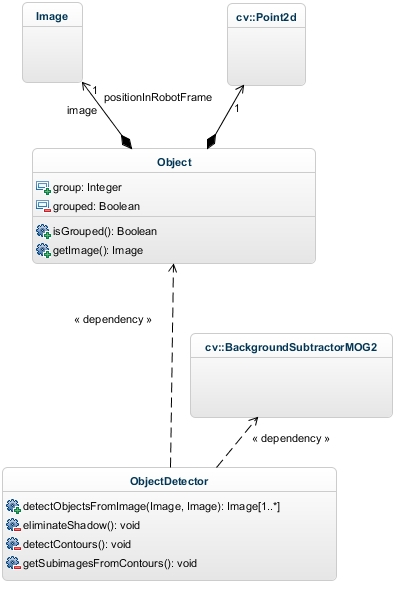
\includegraphics[scale=0.9]{22.eps} 
            \caption{Object Detector classes}
            \label{detector}
        \end{figure}
    % \newpage
        In figure \ref{cluster}, the clustering classes were designed in such a way that other algorithms might be easily added. The abstract class implements the basic functionality and distinguishes the subclasses by names -- an algorithm is identified by its name. 
        \begin{figure}[t!]
            \centering
            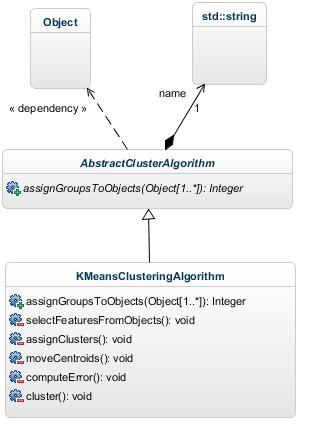
\includegraphics[scale=0.85]{23.eps} 
            \caption{Clustering classes}
            \label{cluster}
        \end{figure}
        In figure \ref{speech} the dependencies of the \verb|Speech| class are shown. This class wraps Text-To-Speech, Speech Recognition and Audio Source Localization functionality. It offers the possibility to speak, hear and determine the approximate position of the speaker.
        \begin{figure}[b!]
            \centering
            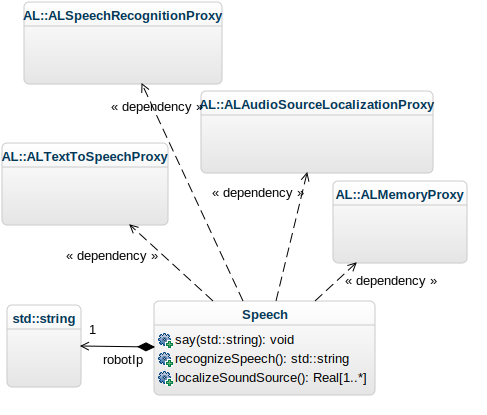
\includegraphics[scale=0.85]{24.eps} 
            \caption{Speech classes}
            \label{speech}
        \end{figure}
% \newpage

        \begin{figure}[b!]
            \centering
            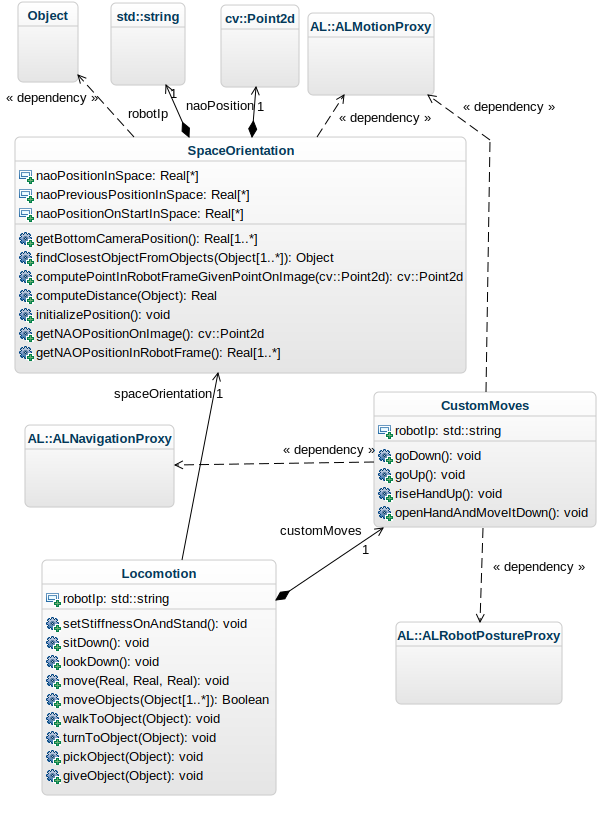
\includegraphics[scale=0.9]{25.eps} 
            \caption{Locomotion and Space Orientation classes}
            \label{locomotion}
        \end{figure}

               In figure \ref{locomotion} it is shown how NAO should perform its movements. But before moving, he needs to know where to move. The class \verb|SpaceOrientation| has this responsibility. The class \verb|SpaceOrientation| is going to be later integrated into \verb|Head| class, while \verb|Locomotion| is more about body itself, so it is a component of \verb|NAO| class, as \verb|Head| itself. But \verb|Locomotion| needs to know about \verb|SpaceOrientation|, so that's why there is an association. The \verb|SpaceOrientation| class computes the distances, performs transformations from one coordinate system to other and retrieves robot's position from sensors. The class \verb|CustomMoves| implements the movements which required Animation Mode to be recorded. Since they are quite specific, they were separated into a different class. Class \verb|Locomotion| has the functionalities like changing robot posture, looking down, perform a generic movement, walk to an object, turn to it, pick it or give it and the method \verb|moveObjects|.
           \begin{figure}[b!]
            \centering
            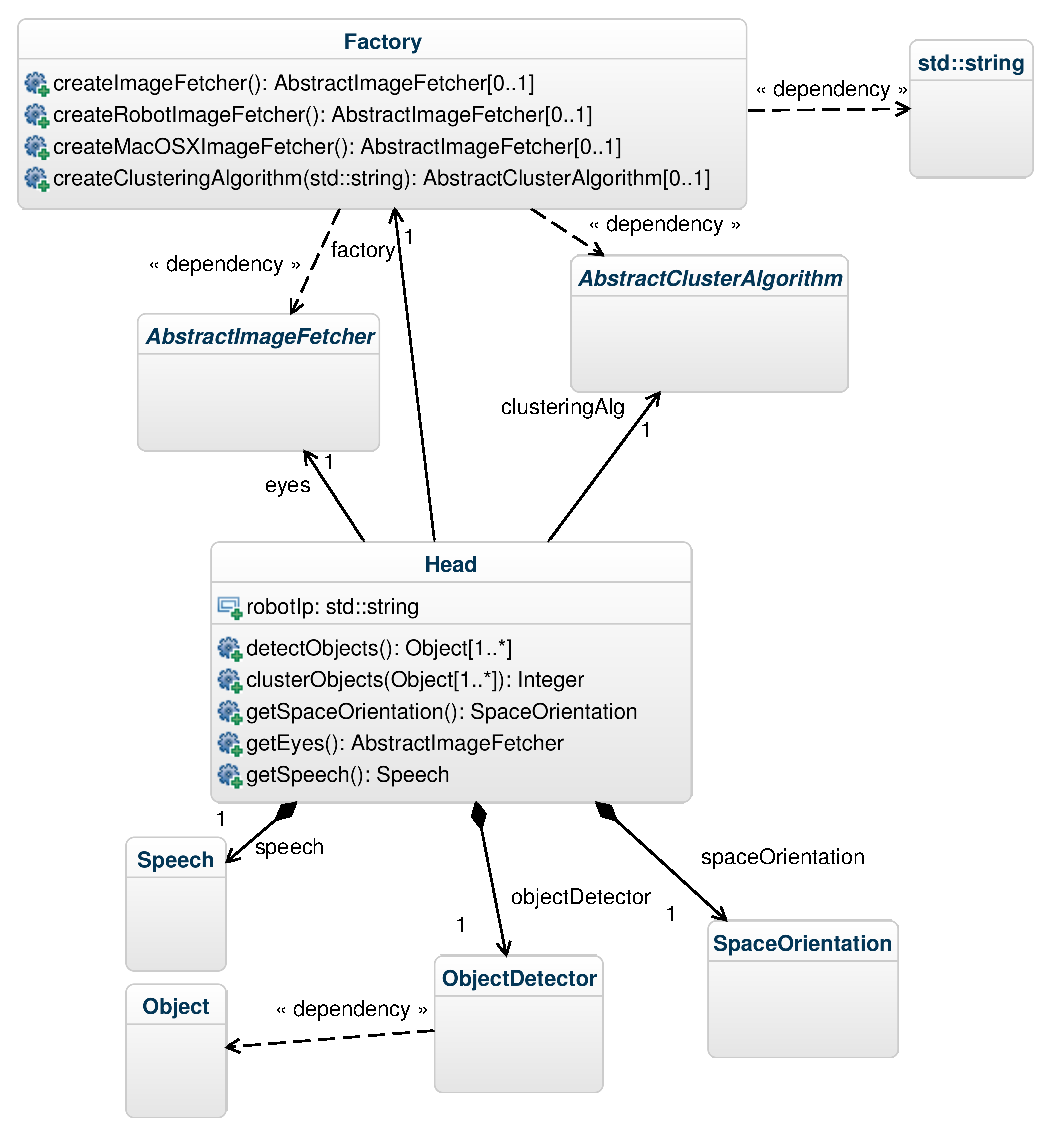
\includegraphics[scale=0.9]{26.eps} 
            \caption{Head class}
            \label{head}
        \end{figure}
        Figure \ref{head} depicts how the class \verb|Head| encapsulates the functionality of speech, object detection and recognition, object clustering and space orientation. At the same time, the \verb|Head| class is decoupled from other specific classes, like \verb|Camera| or a concrete \verb|KMeansClusteringAlgorithm| -- later a different algorithm might be used, or the possibility to choose at runtime the algorithm might be included. That is why the \verb|Factory| design pattern was used. The \verb|Head| class also acts like a facade for the rest, stressing the most important methods of the others. It offers two important methods: \verb|detectObjects| and \verb|clusterObjects|. It also offers access to its members, like \verb|getSpeech| or \verb|getSpaceOrientation|.

        Finally, \ref{naoClass} plays also a role of a facade, but a more general one. It incorporates both \verb|Head| and \verb|Locomotion| and offers functionality like \verb|startInteraction| and \verb|executeCommand|, which are generic for any human-robotic interaction. It also offers public access to its members through getters. 
                To understand how to use these classes and how instances of them interact, the sequence diagram of the whole cycle is presented in figure \ref{sequence} in  Appendix B.
        \begin{figure}[h!]
            \centering
            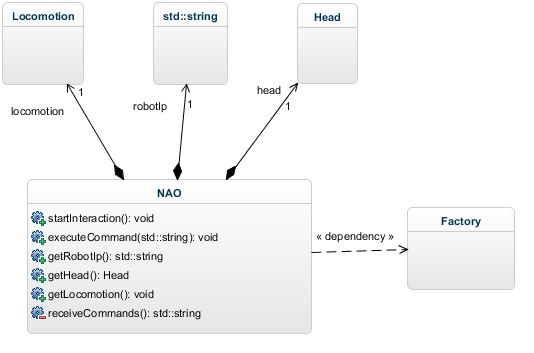
\includegraphics[scale=0.8]{27.jpg} 
            \caption{NAO class}
            \label{naoClass}
        \end{figure}
 

        % \begin{figure}[h!]
        %     \centering
        %     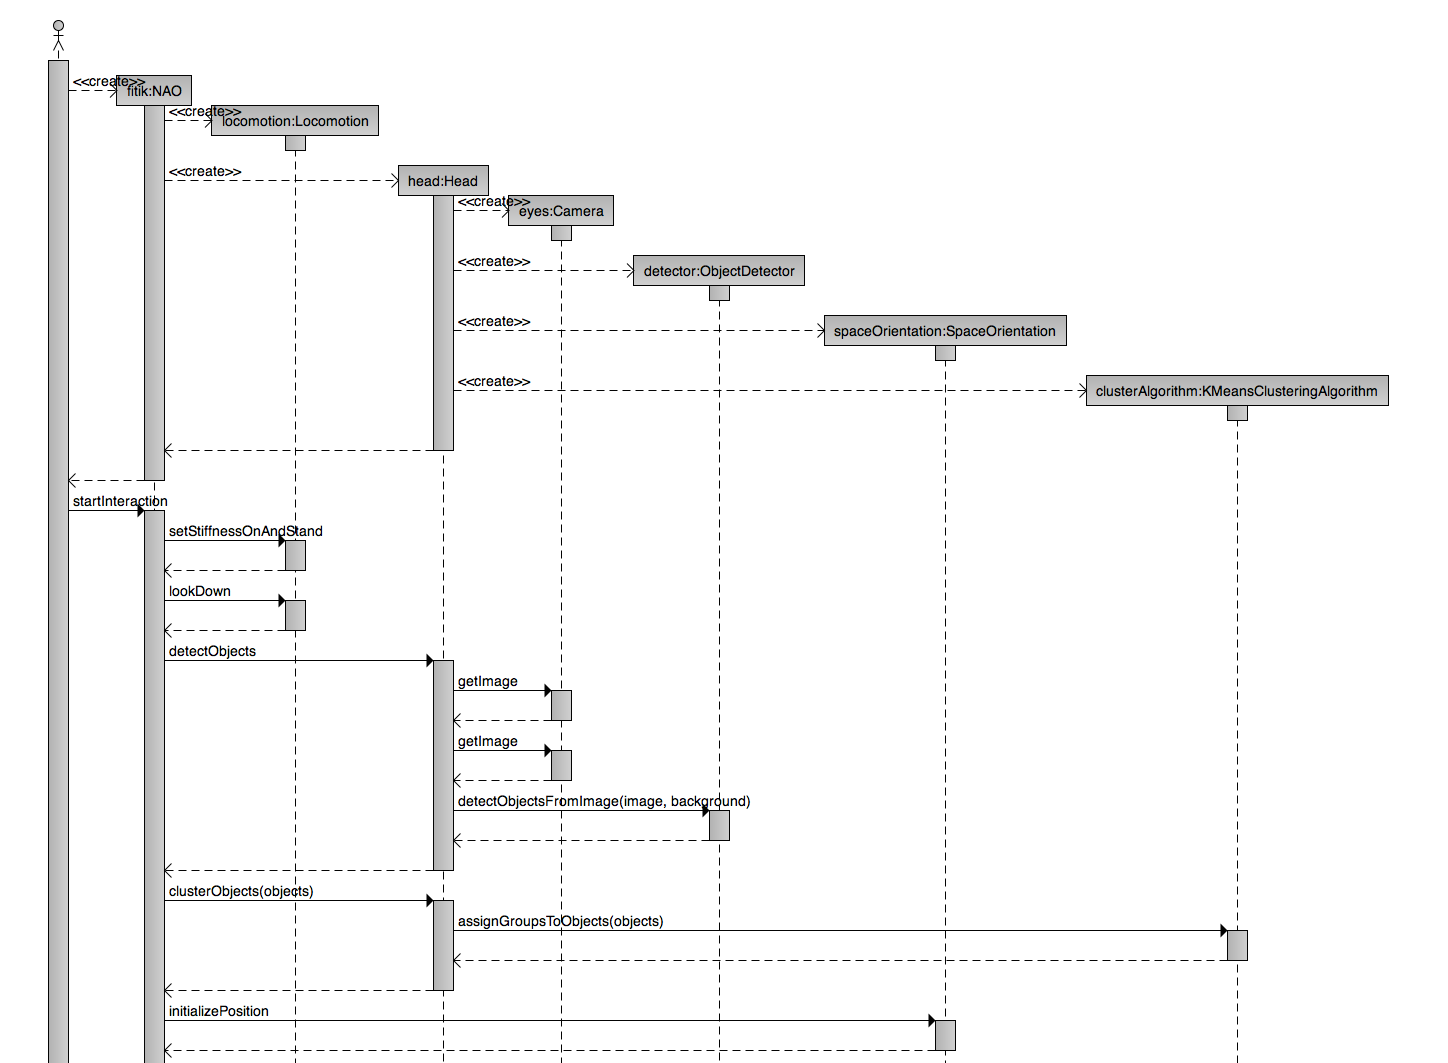
\includegraphics[scale=0.45, angle=90]{28.png} 
        %     \caption{Object interaction -- part I}
        %     \label{sequence1}
        % \end{figure}


        % \begin{figure}[h!]
        %     \centering
        %     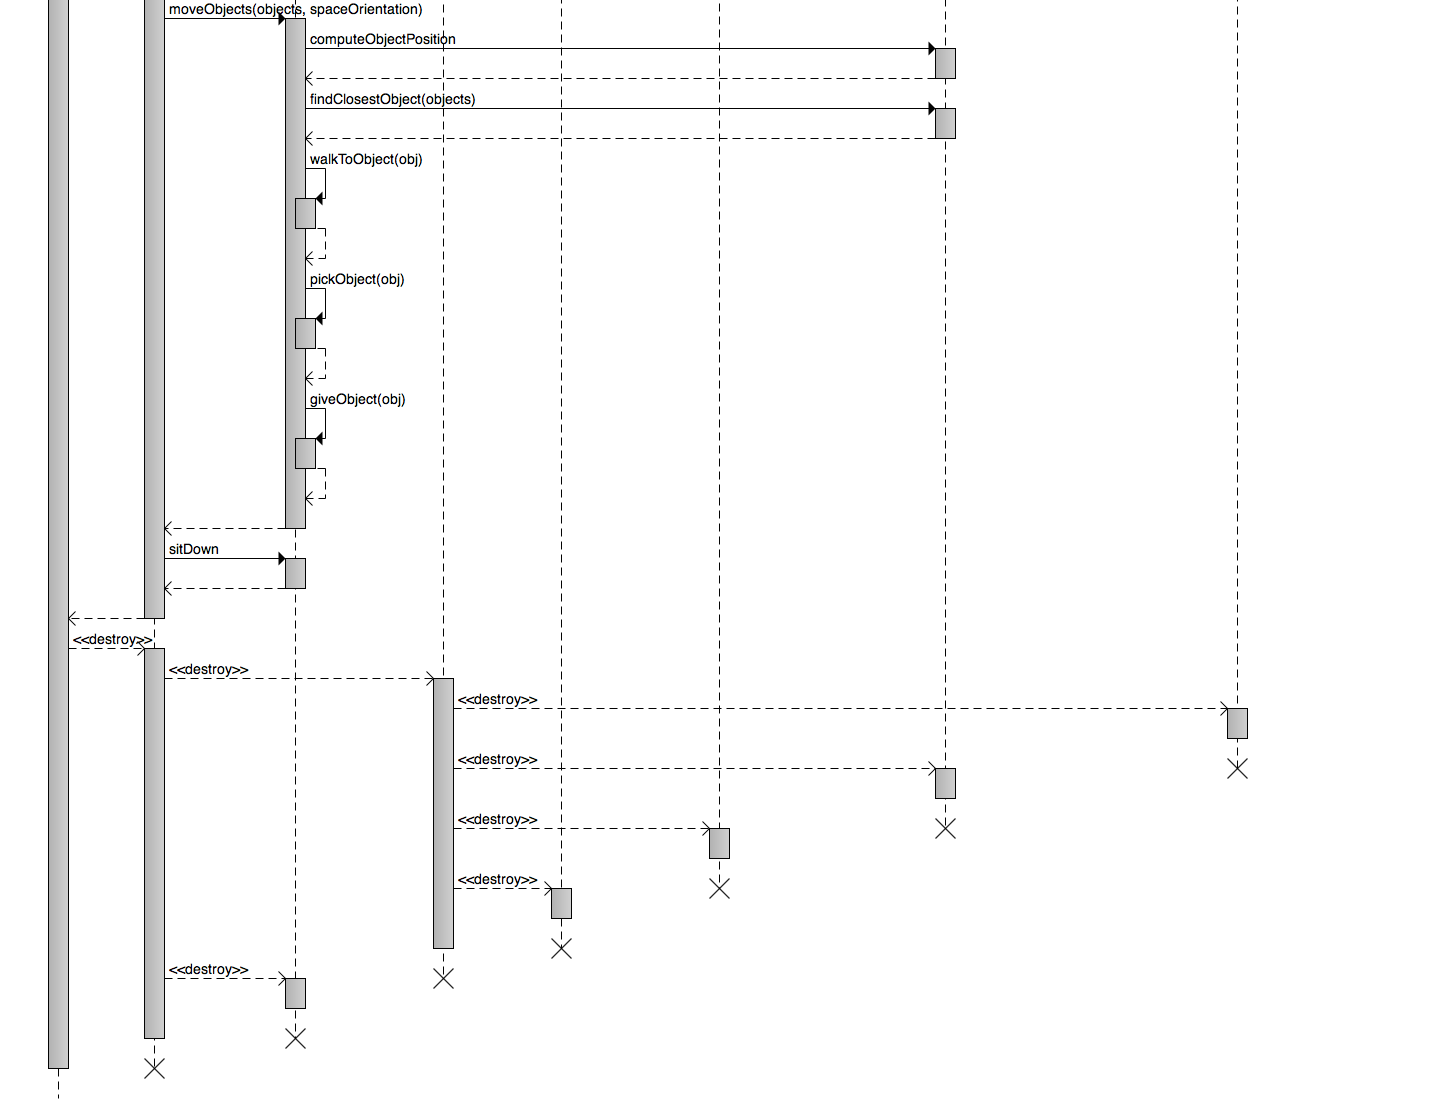
\includegraphics[scale=0.45, angle=90]{29.png} 
        %     \caption{Object interaction -- part II}
        %     \label{sequence2}
        % \end{figure}






\subsection{Implementation}
    \subsubsection{Learning stage}
        Before starting this project, the needed specific technologies and practices should be learned. This project is basically concerned with three topics: NAO robot, OpenCV and Machine Learning. Machine Learning was learned through available free online courses. The first one is available on iTunesU platform, called ``Learning from Data'', tought by professor Yaser Abu-Mostafa, Caltech University. The second one is available from Coursera platform, called ``Machine Learning'', tought by head of Stanford AI lab, Andrew Ng, Stanford University. Both courses include video lectures, slides and homeworks available to download. The only tool required at this stage was Octave, a high-level interpreted language, primarily intended for numerical computations, which is the free version of MatLAB. OpenCV has a great documentation on its official site, with examples and source code. This library is cross-platform, so its installation is the only prerequisite to use it. It was both installed of Linux and Mac OS X.

         NAO was studied using the software which comes with it -- Choreographe. Choreographe has a 90 days free trial period, but also 25 licences are given with the robot. The NAO documentation, available online has a detailed description how to get started or perform some more advanced things with the robot. There is also a community of NAO developers, where different applications are available. So in order to test robot, Choreographe and Webots were installed. Because the C++ SDK is not available for free, Java SDK was used for testing. Later, the installation of C++ SDK have not succeeded on Mac OS X platform. Since Linux was needed anyway and the work was done on two platforms, VirtualBox was installed and a version of Ubuntu on it. On Linux, Qt Creator IDE was installed and additional packages on which the NAO SDK was dependent. After that the C++ SDK was installed and successfully tested. Besides online resources, knowledge was also acquired through discussions with students and consultations with professor Miroslav Skrbek. 

    \subsubsection{Planning}
        The planning of the work was done through asking and answering the right questions. The first two important questions are:
        \begin{enumerate}[topsep=2pt, partopsep=0pt,itemsep=0pt,parsep=1pt]
            \item What the robot can already do;
            \item What the robot cannot do.
        \end{enumerate}
        Studying its capabilities the conclusion was reached, that some actions are very easy to implement, while others are not so intuitive as they may seem (any generic action, not related to this problem). Abstraction is a powerful technique which can be applied for solving any generic engineering problem. Excluding what is irrelevant and leaving only the key points of the problem simplifies it and directs which actions should be done first. Without taking small details into account, there are three subproblems of the main task:
        \begin{enumerate}[topsep=2pt, partopsep=0pt,itemsep=0pt,parsep=1pt]
            \item Detecting an object from the whole picture;
            \item Clustering it;
            \item Moving it.
        \end{enumerate}
        Any subproblem can be divided again in sub-subproblems, recursively, until the current tasks are simple enough to be solved. Then, the solution is built in reverse order, by sticking together the bits. Applying the same Divide \& Conquer method, the following ideas were forumalted:
        \begin{enumerate}[topsep=2pt, partopsep=0pt,itemsep=0pt,parsep=1pt]
            \item teach the system to detect that there are objects; start with one object;
            % \item perform the learning on a computer; the first two steps can be done on a PC, without the need of robot;
            \item teach robot to pick up things;
            \item for increasing the probability of correct matching let him analyze the picked object;
            \item the task is to move the object -- if picking is difficult, object might be dragged.
        \end{enumerate}
        Taking these things into account, the following stages of development were introduced:
        \begin{enumerate}[topsep=2pt, partopsep=0pt,itemsep=0pt,parsep=1pt]
            \item study of Machine Learning -- 1 month;
            \item study of the robot -- 1 month;
            \item study of OpenCV -- 2 weeks;
            \item system design -- 1 week;
            \item system implementation -- 2 months;
            \item testing and analysis -- 2 weeks.
        \end{enumerate}

    \subsubsection{System development}

        The work was started on Mac OS X platform. At the start, Test-Driven Development was used to assure the quality of the code. Latter it was abandoned in favor of time gain. As mentioned, the first two steps did not require the robot so object detection and clustering could be performed on a PC. At first, some draft-programs were written to test the usage of OpenCV. Following some tutorials, it was clear that using \verb|findContours| OpenCV function it is possible to detect the objects. But to detect meant to get their coordinates in the image and the bounding rect so that the sub images might be extracted. Moreover, there were a lot of contours found. Some of them repeated the same shape of one object, some designated just some small dots or shadows -- these were errors. But the \verb|threshold| function gave the possibility to cut dramatically the number of detected contours. As later suggested, many of them were very small, so the filter them one could use the area of that closed contour. The contour could be easily approximated to some polynomial and a polynomial might give the rectangle in which it is enclosed. But detecting objects just from one image was challenging -- that would impose a necessary condition to have a background of one color, without noise. Even with that condition satisfied, the algorithm mistakenly detected shadows as objects. It was a version of detection, which had many disadvantages but it worked.

        After that, a project was created and the basic classes which are indicated in the diagrams were defined, but without a proper implementation yet. It was to assure that the whole skeleton of the application is feasible. A little bit later, this project was added to a git repository, to assure versioning control. A beta-version of object detection was implemented, so the implementation could proceed to the clustering step. Since a custom clustering algorithm was already implemented in MatLAB during online course homeworks, it was ported in C++. Due to the complexity of the real-life machine learning application, the test algorithms are always run on simple points. After different parameters are adjusted, they might be transformed for real examples. Since clustering is Unsupervised Learning, it did not require training. That also meant that it did not require a training data set. At first, the clustering was implemented without Elbow method. The complexity of the implementation of each module was iteratively increased, with each iteration. 


        It was needed to extract somehow features from images. To start simple, only a few were chosen at first iteration. There are as many features as many information bytes in the image. Any pixel of an image can basically be a feature. But due to expensive in processing power algorithms involved in clustering and also due to the fact that clustering itself was repeated many times until the best solution was found, it was unaffordable to use the entire matrix of pixels as features. The simplest way to compare the objects is by comparing their size. So just two features were initially used: the width and the height of the image. An artificial, test image was created with simple shapes as presented in the figure \ref{simpleShape}. The four rectangles, all of the same color but of two different sizes were a good candidate for the start. As the output, OpenCV presented the same image with the detected objects circled with different colors. Each color was associated with a cluster. In a different test, some of the rectangles were rotated by 90 degrees. It caused problems, since the width was associated with the height. Thus all the detected images need first to be preprocessed -- they should be turned in such a way that width is always smaller than the height. 

        % Later, the complexity of the features was increased, taking into account the main colors as well. 

        The implementation of Elbow method was added. It computed the error at every cluster number and looked how dramatically did the error decrease compared to the previous error. The clustering module was tested again with a test image, but this time with different shapes, different colors and multiple clusters. The module successfully determined how many clusters are there and which object goes to which group. Tests also detected numerous wrong groupings, thing which was taken latter into consideration, adjusting the features and other parameters. After the clustering stage was good enough, the module was tested with a real photo. It performed much worse then on simulated images, mostly because of the shadows and light conditions. The problem lay in object detection not in clustering. The background was not so ordinary, it varied from place to place. In a try to tackle that, a method which would recolor the main color was written. It allowed some variance and all the pixels which fell into that range were recolored. That solved the problem but only partially, since now some objects which were slightly of a different color were considered background as well.

        \begin{figure}[t!]
            \centering
            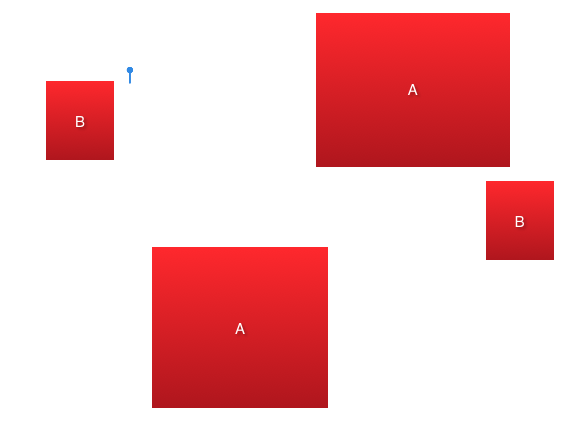
\includegraphics[scale=0.4]{30.png} 
            \caption{Test image for detection and clustering}
            \label{simpleShape}
        \end{figure}

        In the mean time, the project was ported to run on Linux as well, with only difference being the usage of the SDK. The cross-compiled code was written using preprocessing directives, like \verb|#ifdef|. While the program runs on OS X, it retrieves the image from the filesystem and the end result is just a picture with circled objects, sorted in the image. On Linux, program called the needed NAO modules to perform the real moves. So the same modules were tested on NAO, but now the robot retrieved the image from the real camera, and spoke back the results. To test such behavior, the simulator was used. The simulator has limited capabilities, since no speech or its recognition is possible. Another problem was that NAO did not have any grasping functionality implemented. There were no predefined moves for hands and the whole body to reach an object as well. The solution was to use the Animation Mode to define these moves. The robot records the movements of the parts of his body and later they can be reproduced. These movements were then adjusted in Choreographe. The main difficulty in this task is to create such a transition from stand posture to grasping posture that the robot would not fall down during it. Such a movement was obtained only in the last stage of development. 

        After running the project on robot it became obvious that even 50cm for robot are like 2m for a human -- he needs first to walk to an object, then perform that custom movement of grasping. But it was first necessary to know the location of the object in space, in order to know where to move. The analysis of possible ways to compute the distance was done. The most straightforward way is to compute the distance as explained in one of the previous chapters. The height and \( x \) offset of camera were computed from the available sources and robot schemes. Also the corresponding angles were computed. Later a method from SDK which returns these values was used. Since the precision of distance calculation was important, so was the precision of NAO movement. Unfortunately, the precision is quite bad. The robot is biased to the left while moving forward, also performing a small rotation. A small mistake is done during lateral movement as well. Although a compensation of these errors was done, the measurements of errors were not so precise themselves. The errors were a little bit chaotic and it was quite difficult to catch them. This is perhaps the biggest problem still unsolved. 

        After a short research about other functionalities available in OpenCV, it was decided to update the way the objects were detected. It is complicated indeed to make sense what is the background and where are the objects just from one image, especially if the background has some objects drawn on it. The different approach was to use two images -- one of plain background and the next one already with objects. The subtraction is performed and this gives a great mask which can be used later. This method proved to be very good, both independent of background coloring and shadows. After updating the detection method, the system altogether started working better. 

        % The size of the objects which NAO handles and is able to grasp is very small. Not only the size is the problem, but also because of three fingers, some hard solid objects just slide out of his hands while grasping. Only soft objects could be grasped by robot. His fingers are also quite weak and when he tries to close his hand and he meets resistance to this action, he abandons the move. 

        The difference between simulated robot and the real one added some complexity to the task. Some things went quite smoothly in the simulator, but failed on robot. The main problem was the locomotion. Because in the simulator the process was always started from zero the robot was loaded again and all the absolute values which he stores were reset. That is why it was unclear at first that the position which robot retrieves was absolute, but not relative. At every simulation, this absolute position was reset. Because it was reset, all the values indicated zeros and did not influence the distances which robot needed to move. On the other hand, on real robot, these values were not reset and added different biases (being different from zero) and caused the robot to move in almost unpredictable manner. Since this position was not retrieved from the robot's sensors, but by summing up all the previous moves, this data became quite random. It was random because the robot was moved, rotated and transported from place to place by humans -- changes which were not taken into consideration by that data. Finally, the solution was to store the position every time the application run and take it as the origin of coordinates in \verb|FRAME_ROBOT|.

        The robot could detect objects, sort them in some simple way and the basics of locomotion was implemented. At this stage a massive refactoring was done, each class gained a more specific responsibility. The need of some design patterns was revealed. Some abstractions were introduced and common functionality was separated into base classes. To perform the grasping movement, the corresponding movement from Choreographe was exported. The robot was manipulated while the specific positions were recorded. These positions are placed on a timeline and an interpolation between them is done. In such a way, a movement is created. This movement is later exported form Choreographe as a block of code.  

        A set of tests was run to compare the clustering algorithms -- the one available from OpenCV with the one implemented by myself. The tests showed that the library algorithm is better. So the clustering class was updated to use the specific OpenCV functionality. Speech functionality was updated: NAO now said when anything was going wrong. The basics of speech recognition was implemented. Next, the interaction itself with the robot was defined -- everything happens in a infinite loop, in which the robot receives commands and interprets them. The interaction stops when the corresponding command is met. The module with the distance computation was many times updated and changed. Later it was clear that there is no need for the robot to turn (to rotate) -- the way he moves makes him able to reach an object just using the walking feature. 

        The rising of hand was implemented in a similar manner as grasping -- using Animation Mode. It is possible to create such custom movements even without the real robot, but just using the virtual model available in Choreographe. Finally robot successfully traversed the objects. The traversal itself is performed in the following way: NAO selects the closest object to himself and goes to it. It goes down, grasps it and goes up. It gives the object and says to which group it belongs. After that, the process repeats. So in such a way it traverses the objects. But at this stage, NAO does not pick the object, but just goes from one object to other. In the end the grasping functionality was implemented.  This real robot, unlike the one simulated has a error of movement precision. The last stage of development was concerned with compensating these errors, the problem which still remains unsolved. 


    \subsubsection{Results}

        The results show that the project did not achieve its practical goals. The robot was not able to sort the objects due to high mistakes in movement precisions. Nevertheless, during the implementation some interesting achievements were reached. The method of calculation of the distance is both precise and easily reusable in a wide range of tasks. It might be the primitive way to make a robot achieve a 3-D vision. The object detection works flawlessly. It is able to detect objects on almost any background and is able to take shadow into consideration. The illumination though can still affect the result. The clustering is also good, but other algorithms might be used later as well. More features need to be added to make the sorting more elaborate. The system can decide itself the number of clusters. 

        The future work implies refining the current functionality, making the execution local instead of remote and solving the problem of precision. The grasping is difficult due to the number of fingers. The project runs both on Linux and Mac OS X. The Mac OS X functionality needs to be extended, so that remote execution on robot worked from there as well. Similar program should run on Windows platform as well. This project can serve as a detailed analysis of humanoid's capabilities mostly concerned to interaction with objects and humans. This project also presents a successful example of interaction between three components from different branches of IT: robotic functionality, image processing and machine learning. This work itself might be interesting and useful in future robotics research and improvements, both concerned with NAO and other robots as well. 






\clearpage